%%%%%%%%%%%%%%%%%%%%%%%%%%%%%%%%%%%%%%%%%%%%%%%%%%%%%%%%%%%%%%%
%
% Welcome to Overleaf --- just edit your article on the left,
% and we'll compile it for you on the right. If you give 
% someone the link to this page, they can edit at the same
% time. See the help menu above for more info. Enjoy!
%
%%%%%%%%%%%%%%%%%%%%%%%%%%%%%%%%%%%%%%%%%%%%%%%%%%%%%%%%%%%%%%%
%
% For more detailed article preparation guidelines, please see:
% https://f1000research.com/for-authors/article-guidelines/software-tool-articles and http://f1000research.com/data-preparation

\documentclass[9pt,a4paper]{extarticle}
\usepackage{f1000_styles}

%% Default: numerical citations
\usepackage[numbers]{natbib}

%% Uncomment this lines for superscript citations instead
% \usepackage[super]{natbib}

%% Uncomment these lines for author-year citations instead
% \usepackage[round]{natbib}
% \let\cite\citep

%% syntax highlighting style kate 
\renewcommand{\KeywordTok}[1]{\textbf{{#1}}}
\renewcommand{\DataTypeTok}[1]{\textcolor[rgb]{0.50,0.00,0.00}{{#1}}}
\renewcommand{\DecValTok}[1]{\textcolor[rgb]{0.00,0.00,1.00}{{#1}}}
\renewcommand{\BaseNTok}[1]{\textcolor[rgb]{0.00,0.00,1.00}{{#1}}}
\renewcommand{\FloatTok}[1]{\textcolor[rgb]{0.50,0.00,0.50}{{#1}}}
\renewcommand{\ConstantTok}[1]{\textcolor[rgb]{0.00,0.00,0.00}{{#1}}}
\renewcommand{\CharTok}[1]{\textcolor[rgb]{1.00,0.00,1.00}{{#1}}}
\renewcommand{\SpecialCharTok}[1]{\textcolor[rgb]{1.00,0.00,1.00}{{#1}}}
\renewcommand{\StringTok}[1]{\textcolor[rgb]{0.87,0.00,0.00}{{#1}}}
\renewcommand{\VerbatimStringTok}[1]{\textcolor[rgb]{0.87,0.00,0.00}{{#1}}}
\renewcommand{\SpecialStringTok}[1]{\textcolor[rgb]{0.87,0.00,0.00}{{#1}}}
\renewcommand{\ImportTok}[1]{{#1}}
\renewcommand{\CommentTok}[1]{\textcolor[rgb]{0.50,0.50,0.50}{\textit{{#1}}}}
\renewcommand{\DocumentationTok}[1]{\textcolor[rgb]{0.50,0.50,0.50}{\textit{{#1}}}}
\renewcommand{\AnnotationTok}[1]{\textcolor[rgb]{0.50,0.50,0.50}{\textbf{\textit{{#1}}}}}
\renewcommand{\CommentVarTok}[1]{\textcolor[rgb]{0.50,0.50,0.50}{\textbf{\textit{{#1}}}}}
\renewcommand{\OtherTok}[1]{{#1}}
\renewcommand{\FunctionTok}[1]{\textcolor[rgb]{0.00,0.00,0.50}{{#1}}}
\renewcommand{\VariableTok}[1]{{#1}}
\renewcommand{\ControlFlowTok}[1]{{#1}}
\renewcommand{\OperatorTok}[1]{{#1}}
\renewcommand{\BuiltInTok}[1]{{#1}}
\renewcommand{\ExtensionTok}[1]{{#1}}
\renewcommand{\PreprocessorTok}[1]{\textbf{{#1}}}
\renewcommand{\AttributeTok}[1]{{#1}}
\renewcommand{\RegionMarkerTok}[1]{{#1}}
\renewcommand{\InformationTok}[1]{\textcolor[rgb]{0.50,0.50,0.50}{\textbf{\textit{{#1}}}}}
\renewcommand{\WarningTok}[1]{\textcolor[rgb]{1.00,0.00,0.00}{\textbf{{#1}}}}
\renewcommand{\AlertTok}[1]{\textcolor[rgb]{0.00,1.00,0.00}{\textbf{{#1}}}}
\renewcommand{\ErrorTok}[1]{\textcolor[rgb]{1.00,0.00,0.00}{\textbf{{#1}}}}
\renewcommand{\NormalTok}[1]{{#1}}

\begin{document}
\pagestyle{front}

\title{valr: Reproducible genome interval analysis in R}
\author[1]{Kent A. Riemondy}
\author[1]{Austin Gillen}
\author[2]{Ryan M. Sheridan}
\author[2]{Yinni Yu}
\author[3]{Christopher G. Bennett}
\author[1,2,*]{Jay R. Hesselberth}

\affil[1]{University of Colorado School of Medicine, RNA Bioscience Initiative, Aurora CO 80045}
\affil[2]{University of Colorado School of Medicine, Department of Biochemistry and Molecular Genetics}
\affil[3]{ComAnalyzeIT LLC, Fort Collins CO 80525}
\affil[*]{Corresponding author: jay.hesselberth@gmail.com}

\maketitle
\thispagestyle{front}

% 300 words
\begin{abstract}
New tools for genome internal analysis enable analysis of large genomic data sets
Availability of large genomic data sets. Need for new tools for exploratoratory data analysis. valr enables genomic interval analysis in the RStudio environment.
\end{abstract}

\section*{Keywords}

Genomics, Intervals, BEDtools, reproducibility, R, RStudio

\clearpage
\pagestyle{main}
\section*{Introduction}

Determining the correlation between sets of genomic features is a routine task in bioinformatics that requires sophisticated interval arithmetic. Command-line tools for interval analysis such as BEDtools \cite{quinlan_bedtools:_2010} and BEDOPS \cite{neph_bedops:_2012} are powerful tools that are central to many genomic analysis pipelines. A common workflow for genomic analysis begins with preprocessing interval analyses via command-line tools, followed by importing data into R for visualization and further statistical analyses. However, this workflow separation hinders exploratory data analysis, and the development reproducible research workflows built in the RMarkdown framework. 

R packages developed for interval analysis include IRanges \cite{lawrence_software_2013}, GenometriCorr [@Favorov12], and bedr \cite{haider_bedr_2016}. IRanges is a Bioconductor package that provides specialized interval classes and methods to conduct interval arthimetic and is utilized extensively by Bioconductor packages. GenometriCorr provides a set of statistical tests to determine the relationships between interval sets and builds upon IRanges. bedr is a CRAN distributed package that provides wrapper functions to call BEDTools, BedOPS, and tabix functions providing out-of-memory support for interval analysis in R. These packages provide important functionality for interval analysis in R however they do not easily integrate with interactive data visualization features developed for R, such as Shiny\cite{chang_shiny_2017}, and the RStudio IDE. Additionally, the programmatic advances provided by the recent tidyverse suite of data processing and visualization tools (dplyr, purrr, broom, and ggplot2) do not easily interface with the R S4 objects implemented in many Bioconductor packages for data organization \cite{wickham_tidyverse_2017}. 

We therefore sought to develop an R package that allows seamless and extensible interval arithmetic built to incorporate new R programming, visualization, and interactivity features.

\section*{Methods}
\subsection*{Implementation}
valr is implemented as an R package that makes extensive use of dplyr, a popular package that provides a flexible and high-performance framework for data manipulation \cite{wickham_dplyr_2016}. Computationally intensive functions in valr are written in C++ using Rcpp to enable fluid and quick interactive analysis of large datasets\cite{eddelbuettel_rcpp_2011}. 

\subsection*{Operation}
valr is distributed as part of the CRAN R package repository and is compatible with Mac OS X, Windows, and major Linux operating systems. Package dependencies and system requirements are documented on the valr CRAN repository (\url{https://cran.r-project.org/web/packages/valr/index.html}).

\section*{Use Cases} % Optional - only if NO new datasets are included
To demonstrate the functionality and utility of \textbf{valr} presented below are some common use cases for genomic interval analysis. 

\subsection{Basic Usage}

\subsubsection{Input data}\label{input-data}

\texttt{valr} provides a set of functions to read BED, BEDgraph, and VCF into R as convenient \texttt{tbl\_dfs()} dataframe objects. All tbls will have \texttt{chrom}, \texttt{start}, and\texttt{end} columns, and tbls from multi-column formats will have additional pre-determined column names. 

Additionally \texttt{valr} supports connections to remote databases to programatically access the UCSC and Ensembl databases. 

Show examples of read bed with files, url, and readucsc.

\subsection{Terse Syntax}

The functions in \texttt{valr} have similar names to their
\texttt{BEDtools} counterparts, and so will be familiar to users of
the \texttt{BEDtools} suite. 

Similar to pybedtools\cite{dale_pybedtools:_2011}, a python wrapper for BEDTools, valr has a terse syntax. Shown below is an example of how to find all SNPs within 1 Kbp of genes using valr.

\begin{Highlighting}[]
\KeywordTok{library}\NormalTok{(valr)}
\KeywordTok{library}\NormalTok{(dplyr)}

\NormalTok{snps <-}\StringTok{ }\KeywordTok{read_bed}\NormalTok{(}\KeywordTok{valr_example}\NormalTok{(}\StringTok{'hg19.snps147.chr22.bed.gz'}\NormalTok{), }\DataTypeTok{n_fields =} \DecValTok{6}\NormalTok{)}
\NormalTok{genes <-}\StringTok{ }\KeywordTok{read_bed}\NormalTok{(}\KeywordTok{valr_example}\NormalTok{(}\StringTok{'genes.hg19.chr22.bed.gz'}\NormalTok{), }\DataTypeTok{n_fields =} \DecValTok{6}\NormalTok{)}

\CommentTok{# find snps in intergenic regions}
\NormalTok{intergenic <-}\StringTok{ }\KeywordTok{bed_subtract}\NormalTok{(snps, genes)}
\CommentTok{# distance from intergenic snps to nearest gene}
\NormalTok{nearby <-}\StringTok{ }\KeywordTok{bed_closest}\NormalTok{(intergenic, genes)}

\NormalTok{nearby %>%}
\StringTok{  }\KeywordTok{select}\NormalTok{(}\KeywordTok{starts_with}\NormalTok{(}\StringTok{'name'}\NormalTok{), .overlap, .dist) %>%}
\StringTok{  }\KeywordTok{filter}\NormalTok{(}\KeywordTok{abs}\NormalTok{(.dist) <}\StringTok{ }\DecValTok{1000}\NormalTok{)}
\CommentTok{#> # A tibble: 285 x 4}
\CommentTok{#>         name.x            name.y .overlap .dist}
\CommentTok{#>          <chr>             <chr>    <int> <int>}
\CommentTok{#>  1   rs2261631             P704P        0  -267}
\CommentTok{#>  2 rs570770556             POTEH        0  -912}
\CommentTok{#>  3 rs538163832             POTEH        0  -952}
\CommentTok{#>  4   rs9606135            TPTEP1        0  -421}
\CommentTok{#>  5  rs11912392 ANKRD62P1-PARP4P3        0   104}
\CommentTok{#>  6   rs8136454          BC038197        0   355}
\CommentTok{#>  7   rs5992556              XKR3        0  -455}
\CommentTok{#>  8 rs114101676              GAB4        0   473}
\CommentTok{#>  9  rs62236167             CECR7        0   261}
\CommentTok{#> 10   rs5747023             CECR1        0  -386}
\CommentTok{#> # ... with 275 more rows}
\end{Highlighting}

\subsubsection{Visual documentation}\label{visual-documentation}

The \texttt{bed\_glyph()} tool illustrates the results of operations in
\texttt{valr}, similar to those found in the \texttt{BEDtools}
documentation. Shown below is the code to produce glyphs that illustrate the result of intersecting \texttt{x}
and \texttt{y} intervals with \texttt{bed\_intersect()} , and the result of merging \texttt{x} intervals with \texttt{bed\_merge()} (Figure 1 \ref{fig:Figure 1}). 

\begin{Highlighting}[]
\NormalTok{x <-}\StringTok{ }\NormalTok{tibble::}\KeywordTok{tribble}\NormalTok{(}
  \NormalTok{~chrom, ~start, ~end,}
  \StringTok{'chr1'}\NormalTok{, }\DecValTok{25}\NormalTok{,     }\DecValTok{50}\NormalTok{,}
  \StringTok{'chr1'}\NormalTok{, }\DecValTok{100}\NormalTok{,    }\DecValTok{125}
\NormalTok{)}

\NormalTok{y <-}\StringTok{ }\NormalTok{tibble::}\KeywordTok{tribble}\NormalTok{(}
  \NormalTok{~chrom, ~start, ~end,}
  \StringTok{'chr1'}\NormalTok{, }\DecValTok{30}\NormalTok{,     }\DecValTok{75}
\NormalTok{)}

\KeywordTok{bed_glyph}\NormalTok{(}\KeywordTok{bed_intersect}\NormalTok{(x, y))}
\end{Highlighting}

And this glyph illustrates \texttt{bed\_merge()}:

\begin{Highlighting}[]
\NormalTok{x <-}\StringTok{ }\NormalTok{tibble::}\KeywordTok{tribble}\NormalTok{(}
  \NormalTok{~chrom, ~start, ~end,}
  \StringTok{'chr1'}\NormalTok{,      }\DecValTok{1}\NormalTok{,      }\DecValTok{50}\NormalTok{,}
  \StringTok{'chr1'}\NormalTok{,      }\DecValTok{10}\NormalTok{,     }\DecValTok{75}\NormalTok{,}
  \StringTok{'chr1'}\NormalTok{,      }\DecValTok{100}\NormalTok{,    }\DecValTok{120}
\NormalTok{)}

\KeywordTok{bed_glyph}\NormalTok{(}\KeywordTok{bed_merge}\NormalTok{(x))}
\end{Highlighting}

\begin{figure}[!htb]
\centering
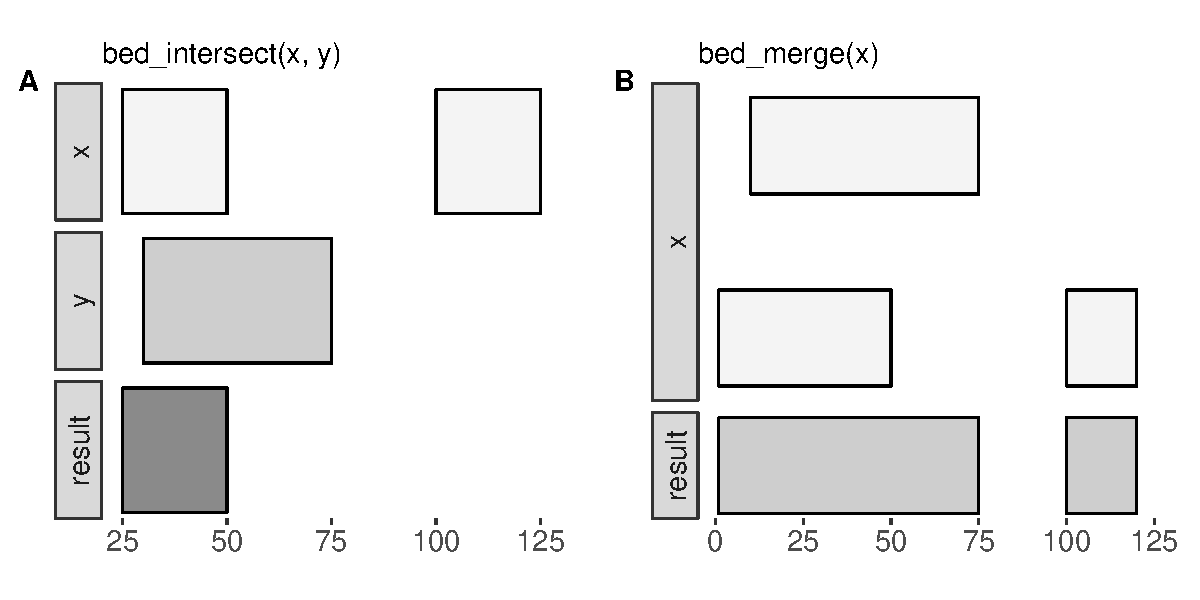
\includegraphics[width=\textwidth]{glyphs.pdf}
\caption{\label{fig:Figure 1}Visualizing interval operations in valr with \texttt{bed\_glyph()}.} 
\end{figure}

\subsubsection{Reproducible reports}\label{reproducible-reports}

\texttt{valr} can be used in RMarkdown documents to generate
reproducible work-flows for data processing. Because \texttt{valr} is
reasonably fast (see the \protect\hyperlink{benchmarks}{benchmarks}), we
now use it in lieu of other tools for exploratory analysis of genomic
data sets in R.

Command-line tools like \texttt{BEDtools} and \texttt{bedops} can be
used in reproducible workflows (e.g., with
\href{https://bitbucket.org/snakemake/snakemake/wiki/Home}{\texttt{snakemake}}),
but it is cumbersome to move from command-line tools to exploratory
analysis and plotting software.
\href{https://pythonhosted.org/pybedtools/}{\texttt{pybedtools}} can be
used within \texttt{ipython\ notebooks} to accomplish a similar goal,
but others have pointed out
\href{https://www.r-bloggers.com/why-i-dont-like-jupyter-fka-ipython-notebook/}{issues
with this approach}, including clunky version control. Because RMarkdown
files are text files, they are readily kept under version control.
Moreover, new features in RStudio, such as notebook viewing, and multiple language support enable similar functionality to \texttt{ipython}.

\subsubsection{Grouping data}\label{grouping-data}

The \texttt{group\_by} function in dplyr can be used to perform functions
on subsets of single and multiple \texttt{data\_frame}s. Functions in
\texttt{valr} leverage grouping to enable a variety of comparisons. For
example, intervals can be grouped by \texttt{strand} to perform
comparisons among intervals on the same strand.

\begin{Highlighting}[]
\NormalTok{x <-}\StringTok{ }\NormalTok{tibble::}\KeywordTok{tribble}\NormalTok{(}
  \NormalTok{~chrom, ~start, ~end, ~strand,}
  \StringTok{'chr1'}\NormalTok{, }\DecValTok{1}\NormalTok{,      }\DecValTok{100}\NormalTok{,  }\StringTok{'+'}\NormalTok{,}
  \StringTok{'chr1'}\NormalTok{, }\DecValTok{50}\NormalTok{,     }\DecValTok{150}\NormalTok{,  }\StringTok{'+'}\NormalTok{,}
  \StringTok{'chr2'}\NormalTok{, }\DecValTok{100}\NormalTok{,    }\DecValTok{200}\NormalTok{,  }\StringTok{'-'}
\NormalTok{)}

\NormalTok{y <-}\StringTok{ }\NormalTok{tibble::}\KeywordTok{tribble}\NormalTok{(}
  \NormalTok{~chrom, ~start, ~end, ~strand,}
  \StringTok{'chr1'}\NormalTok{, }\DecValTok{50}\NormalTok{,     }\DecValTok{125}\NormalTok{,  }\StringTok{'+'}\NormalTok{,}
  \StringTok{'chr1'}\NormalTok{, }\DecValTok{50}\NormalTok{,     }\DecValTok{150}\NormalTok{,  }\StringTok{'-'}\NormalTok{,}
  \StringTok{'chr2'}\NormalTok{, }\DecValTok{50}\NormalTok{,     }\DecValTok{150}\NormalTok{,  }\StringTok{'+'}
\NormalTok{)}

\CommentTok{# intersect tbls by strand}
\NormalTok{x <-}\StringTok{ }\KeywordTok{group_by}\NormalTok{(x, strand)}
\NormalTok{y <-}\StringTok{ }\KeywordTok{group_by}\NormalTok{(y, strand)}

\KeywordTok{bed_intersect}\NormalTok{(x, y)}
\CommentTok{#> # A tibble: 2 x 8}
\CommentTok{#>   chrom start.x end.x strand.x start.y end.y strand.y .overlap}
\CommentTok{#>   <chr>   <dbl> <dbl>    <chr>   <dbl> <dbl>    <chr>    <int>}
\CommentTok{#> 1  chr1       1   100        +      50   125        +       50}
\CommentTok{#> 2  chr1      50   150        +      50   125        +       75}
\end{Highlighting}

Comparisons between intervals on opposite strands are done using the
\texttt{flip\_strands()} function:

\begin{Highlighting}[]
\NormalTok{x <-}\StringTok{ }\KeywordTok{group_by}\NormalTok{(x, strand)}

\NormalTok{y <-}\StringTok{ }\KeywordTok{flip_strands}\NormalTok{(y)}
\NormalTok{y <-}\StringTok{ }\KeywordTok{group_by}\NormalTok{(y, strand)}

\KeywordTok{bed_intersect}\NormalTok{(x, y)}
\CommentTok{#> # A tibble: 3 x 8}
\CommentTok{#>   chrom start.x end.x strand.x start.y end.y strand.y .overlap}
\CommentTok{#>   <chr>   <dbl> <dbl>    <chr>   <dbl> <dbl>    <chr>    <int>}
\CommentTok{#> 1  chr2     100   200        -      50   150        -       50}
\CommentTok{#> 2  chr1       1   100        +      50   150        +       50}
\CommentTok{#> 3  chr1      50   150        +      50   150        +      100}
\end{Highlighting}

Both single set (e.g. \texttt{bed\_merge()}) and multi set operations
will respect groupings in the input intervals.

\subsubsection{Column specification}\label{column-specification}

Columns in \texttt{BEDtools} are referred to by position:

\begin{Shaded}
\begin{Highlighting}[]
\CommentTok{# calculate the mean of column 6 for intervals in `b` that overlap with `a`}
\KeywordTok{bedtools} \NormalTok{map -a a.bed -b b.bed -c 6 -o mean}
\end{Highlighting}
\end{Shaded}

In \texttt{valr}, columns are referred to by name and can be used in
multiple name/value expressions for summaries.

\begin{Shaded}
\begin{Highlighting}[]
\CommentTok{# calculate the mean and variance for a `value` column}
\KeywordTok{bed_map}\NormalTok{(a, b, }\DataTypeTok{.mean =} \KeywordTok{mean}\NormalTok{(value), }\DataTypeTok{.var =} \KeywordTok{var}\NormalTok{(value))}

\CommentTok{# report concatenated and max values for merged intervals}
\KeywordTok{bed_merge}\NormalTok{(a, }\DataTypeTok{.concat =} \KeywordTok{concat}\NormalTok{(value), }\DataTypeTok{.max =} \KeywordTok{max}\NormalTok{(value))}
\end{Highlighting}
\end{Shaded}


\subsection{API}\label{api}
The major functions available in valr are shown in Table \ref{tab:tools}. 

\begin{table}[h!]
\hrule \vspace{0.1cm}
\caption{\label{tab:tools} An overview of major functions available in valr.}
\centering
\begin{tabular}{lr}
 \bfseries \large Function Name & \bfseries  \large Purpose \\ 
  \hline
\bfseries Reading Data & \\ 
  read\_bed & Read BED files \\ 
  read\_bedgraph & Read bedGraph files \\
  read\_narrowpeak & Read narrowPeak files \\
  read\_broadpeak & Read broadPeak files \\
\bfseries Interval Transformation \\ 
  bed\_slop & Expand interval coordinates \\
  bed\_shift & Shift interval coordinates \\
  bed\_flank & Create flanking intervals \\
  bed\_merge & Merge overlapping intervals \\
  bed\_cluster & Identify (but not merge) overlapping intervals \\
  bed\_complement & Create intervals not covered by a query \\
\bfseries Interval Comparison & \\ 
  bed\_intersect & Report intersecting intervals from x and y tbls \\ 
  bed\_cluster & Cluster neighboring intervals \\
  bed\_map & Apply functions to selected columns for overlapping intervals \\
  bed\_subtract & Remove intervals based on overlaps \\
  bed\_window & Find overlapping intervals within a window \\
  bed\_closest & Find the closest intervals independent of overlaps \\
\bfseries Randomizing intervals & \\
  bed\_random & Generate random intervals from an input genome \\
  bed\_shuffle & Shuffle the coordinates of input intervals \\
\bfseries Interval statistics & \\
  bed\_fisher, bed\_projection & Calculate significance of overlaps between two sets of intervals \\
  bed\_reldist & Quantify relative distances between sets of intervals \\
  bed\_absdist & Quantify absolute distances between sets of intervals \\
  bed\_jaccard &Quantify extent of overlap between two sets of intervals \\
\bfseries Utilities &  \\ 
  bed\_glyph & Visualize the actions of valr functions \\ 
  bound\_intervals & Constrain intervals to a genome reference \\
  bed\_makewindows & Subdivide intervals \\
  bed12\_to\_exons & Convert BED12 to BED6 format \\
  interval\_spacing & Calculate spacing between intervals \\
  db\_ucsc, db\_ensembl & Access remote databases \\
  \end{tabular}
\end{table}

\subsection*{Summarizing interval coverage across genomic features}

This demonstration illustrates how to use \texttt{valr} tools to perform
a ``meta-analysis'' of signals relative to genomic features. Here we to
analyze the distribution of histone marks surrounding transcription
start sites.

First we load libraries and relevant data.

\begin{Highlighting}[]
\CommentTok{# `valr_example()` identifies the path of example files}
\NormalTok{bedfile <-}\StringTok{ }\KeywordTok{valr_example}\NormalTok{(}\StringTok{'genes.hg19.chr22.bed.gz'}\NormalTok{)}
\NormalTok{genomefile <-}\StringTok{ }\KeywordTok{valr_example}\NormalTok{(}\StringTok{'hg19.chrom.sizes.gz'}\NormalTok{)}
\NormalTok{bgfile  <-}\StringTok{ }\KeywordTok{valr_example}\NormalTok{(}\StringTok{'hela.h3k4.chip.bg.gz'}\NormalTok{)}

\NormalTok{genes <-}\StringTok{ }\KeywordTok{read_bed}\NormalTok{(bedfile, }\DataTypeTok{n_fields =} \DecValTok{6}\NormalTok{)}
\NormalTok{genome <-}\StringTok{ }\KeywordTok{read_genome}\NormalTok{(genomefile)}
\NormalTok{y <-}\StringTok{ }\KeywordTok{read_bedgraph}\NormalTok{(bgfile)}
\end{Highlighting}

Then we generate 1 bp intervals to represent transcription start sites
(TSSs). We focus on \texttt{+} strand genes, but \texttt{-} genes are
easily accomodated by filtering them and using
\texttt{bed\_makewindows()} with \texttt{reverse}d window numbers.

\begin{Highlighting}[]
\CommentTok{# generate 1 bp TSS intervals, `+` strand only}
\NormalTok{tss <-}\StringTok{ }\NormalTok{genes %>%}
\StringTok{  }\KeywordTok{filter}\NormalTok{(strand ==}\StringTok{ '+'}\NormalTok{) %>%}
\StringTok{  }\KeywordTok{mutate}\NormalTok{(}\DataTypeTok{end =} \NormalTok{start +}\StringTok{ }\DecValTok{1}\NormalTok{)}

\CommentTok{# 1000 bp up and downstream}
\NormalTok{region_size <-}\StringTok{ }\DecValTok{1000}
\CommentTok{# 50 bp windows}
\NormalTok{win_size <-}\StringTok{ }\DecValTok{50}

\CommentTok{# add slop to the TSS, break into windows and add a group}
\NormalTok{x <-}\StringTok{ }\NormalTok{tss %>%}
\StringTok{  }\KeywordTok{bed_slop}\NormalTok{(genome, }\DataTypeTok{both =} \NormalTok{region_size) %>%}
\StringTok{  }\KeywordTok{bed_makewindows}\NormalTok{(genome, win_size)}

\NormalTok{x}
\CommentTok{#> # A tibble: 13,530 x 7}
\CommentTok{#>    chrom    start      end      name score strand .win_id}
\CommentTok{#>    <chr>    <int>    <int>     <chr> <chr>  <chr>   <int>}
\CommentTok{#>  1 chr22 16161065 16161115 LINC00516     3      +       1}
\CommentTok{#>  2 chr22 16161115 16161165 LINC00516     3      +       2}
\CommentTok{#>  3 chr22 16161165 16161215 LINC00516     3      +       3}
\CommentTok{#>  4 chr22 16161215 16161265 LINC00516     3      +       4}
\CommentTok{#>  5 chr22 16161265 16161315 LINC00516     3      +       5}
\CommentTok{#>  6 chr22 16161315 16161365 LINC00516     3      +       6}
\CommentTok{#>  7 chr22 16161365 16161415 LINC00516     3      +       7}
\CommentTok{#>  8 chr22 16161415 16161465 LINC00516     3      +       8}
\CommentTok{#>  9 chr22 16161465 16161515 LINC00516     3      +       9}
\CommentTok{#> 10 chr22 16161515 16161565 LINC00516     3      +      10}
\CommentTok{#> # ... with 13,520 more rows}
\end{Highlighting}

Now we use the \texttt{.win\_id} group with \texttt{bed\_map()} to
caluclate a sum by mapping \texttt{y} signals onto the intervals in
\texttt{x}. These data are regrouped by \texttt{.win\_id} and a summary
with \texttt{mean} and \texttt{sd} values is calculated.

\begin{Highlighting}[]
\CommentTok{# map signals to TSS regions and calculate summary statistics.}
\NormalTok{res <-}\StringTok{ }\KeywordTok{bed_map}\NormalTok{(x, y, }\DataTypeTok{win_sum =} \KeywordTok{sum}\NormalTok{(value, }\DataTypeTok{na.rm =} \OtherTok{TRUE}\NormalTok{)) %>%}
\StringTok{  }\KeywordTok{group_by}\NormalTok{(.win_id) %>%}
\StringTok{  }\KeywordTok{summarize}\NormalTok{(}\DataTypeTok{win_mean =} \KeywordTok{mean}\NormalTok{(win_sum, }\DataTypeTok{na.rm =} \OtherTok{TRUE}\NormalTok{),}
            \DataTypeTok{win_sd =} \KeywordTok{sd}\NormalTok{(win_sum, }\DataTypeTok{na.rm =} \OtherTok{TRUE}\NormalTok{))}

\NormalTok{res}
\CommentTok{#> # A tibble: 41 x 3}
\CommentTok{#>    .win_id win_mean    win_sd}
\CommentTok{#>      <int>    <dbl>     <dbl>}
\CommentTok{#>  1       1 100.8974  85.83423}
\CommentTok{#>  2       2 110.6829  81.13521}
\CommentTok{#>  3       3 122.9070  99.09635}
\CommentTok{#>  4       4 116.2800  96.30098}
\CommentTok{#>  5       5 116.3500 102.33773}
\CommentTok{#>  6       6 124.9048  95.08887}
\CommentTok{#>  7       7 122.9437  94.39792}
\CommentTok{#>  8       8 127.5946  91.47407}
\CommentTok{#>  9       9 130.2051  95.71309}
\CommentTok{#> 10      10 130.1220  88.82809}
\CommentTok{#> # ... with 31 more rows}
\end{Highlighting}

Finally, these summary statistics are used to construct a plot that
illustrates histone density surrounding TSSs (Figure 2\ref{fig:Figure 2}).

\begin{Highlighting}[]
\KeywordTok{library}\NormalTok{(ggplot2)}

\NormalTok{x_labels <-}\StringTok{ }\KeywordTok{seq}\NormalTok{(-region_size, region_size, }\DataTypeTok{by =} \NormalTok{win_size *}\StringTok{ }\DecValTok{5}\NormalTok{)}
\NormalTok{x_breaks <-}\StringTok{ }\KeywordTok{seq}\NormalTok{(}\DecValTok{1}\NormalTok{, }\DecValTok{41}\NormalTok{, }\DataTypeTok{by =} \DecValTok{5}\NormalTok{)}

\NormalTok{sd_limits <-}\StringTok{ }\KeywordTok{aes}\NormalTok{(}\DataTypeTok{ymax =} \NormalTok{win_mean +}\StringTok{ }\NormalTok{win_sd, }\DataTypeTok{ymin =} \NormalTok{win_mean -}\StringTok{ }\NormalTok{win_sd)}

\KeywordTok{ggplot}\NormalTok{(res, }\KeywordTok{aes}\NormalTok{(}\DataTypeTok{x =} \NormalTok{.win_id, }\DataTypeTok{y =} \NormalTok{win_mean)) +}
\StringTok{  }\KeywordTok{geom_point}\NormalTok{() +}\StringTok{ }\KeywordTok{geom_pointrange}\NormalTok{(sd_limits) +}\StringTok{ }
\StringTok{  }\KeywordTok{scale_x_continuous}\NormalTok{(}\DataTypeTok{labels =} \NormalTok{x_labels, }\DataTypeTok{breaks =} \NormalTok{x_breaks) +}\StringTok{ }
\StringTok{  }\KeywordTok{xlab}\NormalTok{(}\StringTok{'Position (bp from TSS)'}\NormalTok{) +}\StringTok{ }\KeywordTok{ylab}\NormalTok{(}\StringTok{'Signal'}\NormalTok{) +}\StringTok{ }
\StringTok{  }\KeywordTok{ggtitle}\NormalTok{(}\StringTok{'Human H3K4me3 signal near transcription start sites'}\NormalTok{) +}
\StringTok{  }\KeywordTok{theme_classic}\NormalTok{()}
\end{Highlighting}


\begin{figure}[!htb]
\centering
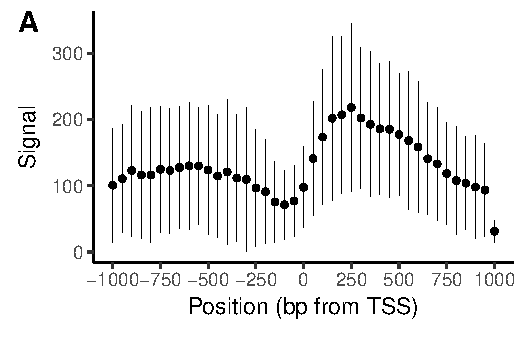
\includegraphics[width=\textwidth]{tss.pdf}
\caption{\label{fig:Figure 2}Meta-analysis of signals relative to genomic features with valr. \textnormal{Summarized coverage of human H3K4Me3 Chip-Seq coverage across positive strand transcription start sites. Data presented +/- SEM.}}
\end{figure}


\subsection*{Interval statistics}\label{interval-statistics}

Estimates of significance for interval overlaps can be obtained by
combining \texttt{bed\_shuffle()}, \texttt{bed\_random()} and the
\texttt{sample\_} functions from \texttt{dplyr} with interval statistics
in \texttt{valr}.

Here we examine the overlap of repeat classes in the human genome (on
\texttt{chr22} only, for simplicity) using \texttt{bed\_jaccard()}.

\begin{Highlighting}[]
\KeywordTok{library}\NormalTok{(purrr)}
\KeywordTok{library}\NormalTok{(tidyr)}

\NormalTok{repeats <-}\StringTok{ }\KeywordTok{read_bed}\NormalTok{(}\KeywordTok{valr_example}\NormalTok{(}\StringTok{'hg19.rmsk.chr22.bed.gz'}\NormalTok{), }\DataTypeTok{n_fields =} \DecValTok{6}\NormalTok{) }
\NormalTok{genome <-}\StringTok{ }\KeywordTok{read_genome}\NormalTok{(}\KeywordTok{valr_example}\NormalTok{(}\StringTok{'hg19.chrom.sizes.gz'}\NormalTok{))}


\NormalTok{shuffle_intervals <-}\StringTok{ }\NormalTok{function(n, .data, genome) \{}
  \KeywordTok{replicate}\NormalTok{(n, }\KeywordTok{bed_shuffle}\NormalTok{(.data, genome, }\DataTypeTok{seed =} \DecValTok{1010486}\NormalTok{), }\DataTypeTok{simplify =} \OtherTok{FALSE}\NormalTok{) %>%}
\StringTok{    }\KeywordTok{bind_rows}\NormalTok{(}\DataTypeTok{.id =} \StringTok{'rep'}\NormalTok{) %>%}
\StringTok{    }\KeywordTok{group_by}\NormalTok{(rep) %>%}\StringTok{ }\KeywordTok{nest}\NormalTok{()}
\NormalTok{\}}

\NormalTok{shuffled <-}\StringTok{ }\KeywordTok{shuffle_intervals}\NormalTok{(}\DataTypeTok{n =} \DecValTok{100}\NormalTok{, repeats, genome) %>%}
\StringTok{  }\KeywordTok{mutate}\NormalTok{(}\DataTypeTok{jaccard =} \NormalTok{data %>%}
\StringTok{           }\KeywordTok{map}\NormalTok{(bed_jaccard, repeats) %>%}
\StringTok{           }\KeywordTok{map_dbl}\NormalTok{(}\StringTok{"jaccard"}\NormalTok{))}
  
\NormalTok{shuffled}
\CommentTok{#> # A tibble: 100 x 3}
\CommentTok{#>      rep                  data      jaccard}
\CommentTok{#>    <chr>                <list>        <dbl>}
\CommentTok{#>  1     1 <tibble [10,000 x 6]> 0.0004355887}
\CommentTok{#>  2     2 <tibble [10,000 x 6]> 0.0004355887}
\CommentTok{#>  3     3 <tibble [10,000 x 6]> 0.0004355887}
\CommentTok{#>  4     4 <tibble [10,000 x 6]> 0.0004355887}
\CommentTok{#>  5     5 <tibble [10,000 x 6]> 0.0004355887}
\CommentTok{#>  6     6 <tibble [10,000 x 6]> 0.0004355887}
\CommentTok{#>  7     7 <tibble [10,000 x 6]> 0.0004355887}
\CommentTok{#>  8     8 <tibble [10,000 x 6]> 0.0004355887}
\CommentTok{#>  9     9 <tibble [10,000 x 6]> 0.0004355887}
\CommentTok{#> 10    10 <tibble [10,000 x 6]> 0.0004355887}
\CommentTok{#> # ... with 90 more rows}
\end{Highlighting}

\subsection*{Analysis of DNA methylation}

\subsection*{Benchmarking against bedtools}
In order to ensure that valr performs fast enough to enable interactive analysis, key functionality is implemented in C++. We benchmarked major valr functions against corresponding commands in BEDTools. valr operates on tables already preloaded into RAM, whereas BEDTools performs file-reading, processing, and writing. To compare valr against bedtools we generated two files containing 1 million random 1 Kbp intervals derived from the human genome. For valr functions, we timed reading the table into R (e.g. with read\_bed()) and performing the respective function. For BEDTools commands we timed executing the command with the output written to /dev/null. valr functions performed similarly or slightly faster than BEDTools commands with the exception of the bed\_map and bed\_fisher (Figure 3\ref{fig:Figure 3}) . 

\begin{figure}[!htb]
\centering
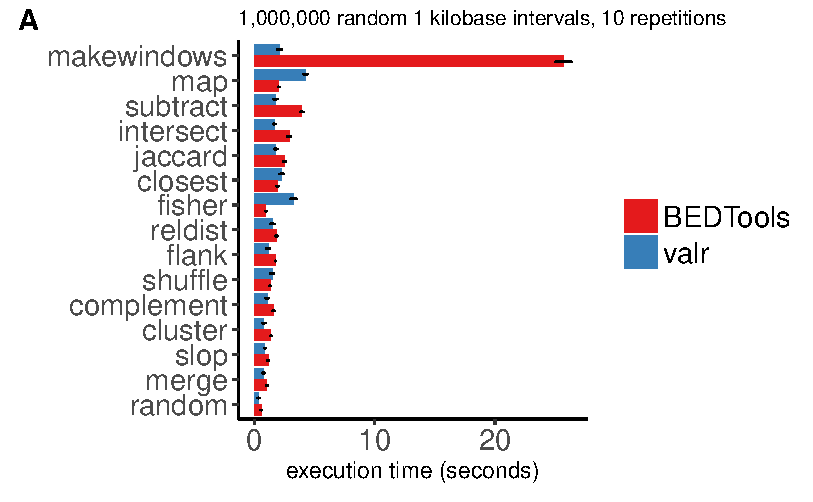
\includegraphics[width=\textwidth]{benchmarks.pdf}
\caption{\label{fig:Figure 3} Performance of major valr functionality benchmarked against BEDTools \textnormal{Timings calculated using microbenchmark and GNU time commands for valr and BEDTools respectively (A).}}
\end{figure}

\section*{Summary} % Optional - only if NO new datasets are included
valr provides a flexible framework for interval arithmetic in R/Rstudio. valr functions are written with a simple and terse syntax that promotes flexible interactive analysis. Additionally by providing an easy-to-use interface for interval arithmetic in R, valr is also a useful teaching tool to introduce the analyses necessary to investigate correlations between genomic intervals, without requiring familiarity with the command-line.

bedr provides a complementary set of tools for working with datasets where RAM limits loading all data into R. IRanges, is a mature package, but is a different philsophy. valr provides some of the functionality of Genometricorr, nbut is extensible to additional statistical test. 

\section*{Software availability}
\begin{enumerate}
\item URL valr can be installed via CRAN using "install.packages('valr')". 
\item valr is maintained at http://github.com/rnabioco/valr
\item valr source code is available at http://github.com/rnabioco/valr
\item Latest stable version of source code is at: https://github.com/rnabioco/valr/archive/v0.2.0.tar.gz TO UPDATE
\item Software license: MIT 
\end{enumerate}

\section*{Author contributions}
In order to give appropriate credit to each author of an article, the individual
contributions of each author to the manuscript should be detailed in this section. We
recommend using author initials and then stating briefly how they contributed.

\section*{Competing interests}
No competing interests were disclosed

\section*{Grant information}
This work was supported by the RNA Bioscience Initiative (funded by a Transformational Research Award from the University of Colorado School of Medicine) and a grant from the National Institutes of Health (XXX to J.H.)

\section*{Acknowledgments}
This work was in part completed during an NIH sponsored Hackathon hosted by the Biofrontiers Department at the University of Colorado at Boulder. 

{\small\bibliographystyle{unsrtnat}
\bibliography{valr}}

\section*{Figures}

\begin{figure}
\centering
    \begin{subfigure}[b]{0.45\textwidth}
\begin{Shaded}
\begin{Highlighting}[]
\NormalTok{x <-}\StringTok{ }\KeywordTok{trbl_interval}\NormalTok{(}
  \NormalTok{~chrom, ~start, ~end,}
  \StringTok{'chr1'}\NormalTok{, }\DecValTok{25}\NormalTok{,     }\DecValTok{50}\NormalTok{,}
  \StringTok{'chr1'}\NormalTok{, }\DecValTok{100}\NormalTok{,    }\DecValTok{125}
\NormalTok{)}

\NormalTok{y <-}\StringTok{ }\KeywordTok{trbl_interval}\NormalTok{(}
  \NormalTok{~chrom, ~start, ~end,}
  \StringTok{'chr1'}\NormalTok{, }\DecValTok{30}\NormalTok{,     }\DecValTok{75}
\NormalTok{)}

\KeywordTok{bed_glyph}\NormalTok{(}\KeywordTok{bed_intersect}\NormalTok{(x, y))}
\end{Highlighting}
\end{Shaded}
        \label{fig:bed_glyph_code}
    \end{subfigure}
    ~
\begin{subfigure}[b]{0.45\textwidth}
        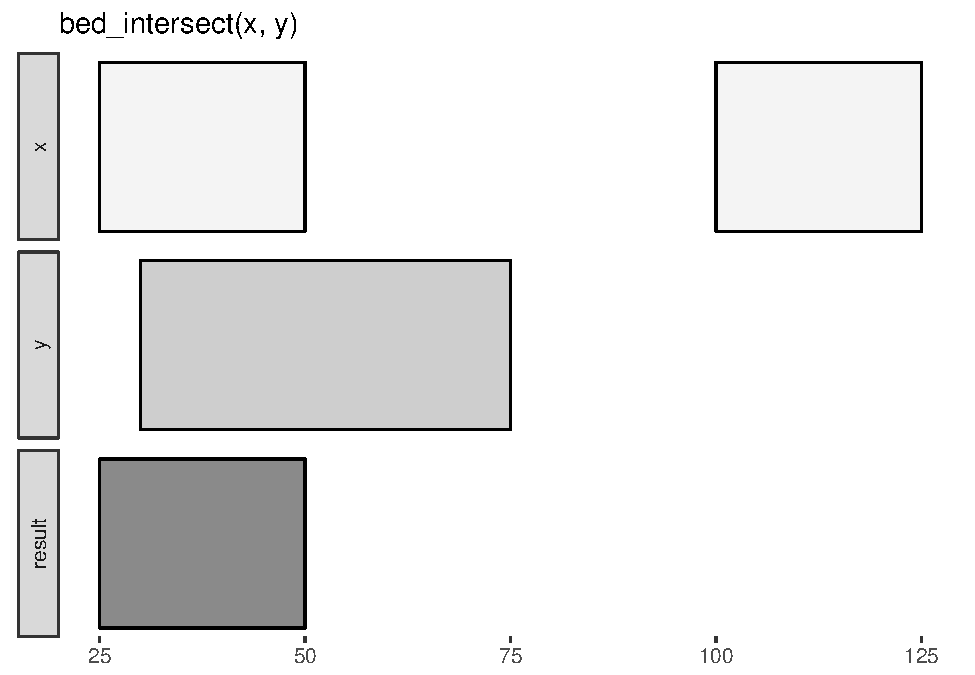
\includegraphics[width=\textwidth]{intersect_glyph-1.pdf}
        \label{fig:bed_glyph_out}
    \end{subfigure}
\caption{\label{fig:your-figure}Visualizing interval intersections with valr.	 }
\end{figure}

\begin{figure}
\centering
    \begin{subfigure}[b]{\textwidth}
\begin{Shaded}
\begin{Highlighting}[]
\CommentTok{# `valr_example()` identifies the path of example files}
\NormalTok{bedfile <-}\StringTok{ }\KeywordTok{valr_example}\NormalTok{(}\StringTok{'genes.hg19.chr22.bed.gz'}\NormalTok{)}
\NormalTok{genomefile <-}\StringTok{ }\KeywordTok{valr_example}\NormalTok{(}\StringTok{'hg19.chrom.sizes.gz'}\NormalTok{)}
\NormalTok{bgfile  <-}\StringTok{ }\KeywordTok{valr_example}\NormalTok{(}\StringTok{'hela.h3k4.chip.bg.gz'}\NormalTok{)}

\NormalTok{genes <-}\StringTok{ }\KeywordTok{read_bed}\NormalTok{(bedfile, }\DataTypeTok{n_fields =} \DecValTok{6}\NormalTok{)}
\NormalTok{genome <-}\StringTok{ }\KeywordTok{read_genome}\NormalTok{(genomefile)}
\NormalTok{y <-}\StringTok{ }\KeywordTok{read_bedgraph}\NormalTok{(bgfile)}

\CommentTok{# generate 1 bp TSS intervals, `+` strand only}
\NormalTok{tss <-}\StringTok{ }\NormalTok{genes %>%}\StringTok{ }\KeywordTok{filter}\NormalTok{(strand ==}\StringTok{ '+'}\NormalTok{) %>%}\StringTok{ }\KeywordTok{mutate}\NormalTok{(}\DataTypeTok{end =} \NormalTok{start +}\StringTok{ }\DecValTok{1}\NormalTok{)}

\CommentTok{# 1000 bp up and downstream}
\NormalTok{region_size <-}\StringTok{ }\DecValTok{1000}

\CommentTok{# 50 bp windows}
\NormalTok{win_size <-}\StringTok{ }\DecValTok{50}

\CommentTok{# add slop to the TSS, break into windows and add a group}
\NormalTok{x <-}\StringTok{ }\NormalTok{tss %>%}\StringTok{ }\KeywordTok{bed_slop}\NormalTok{(genome, }\DataTypeTok{both =} \NormalTok{region_size) %>%}
\StringTok{  }\KeywordTok{bed_makewindows}\NormalTok{(genome, win_size)}

\CommentTok{# map signals to TSS regions and calculate summary statistics.}
\NormalTok{res <-}\StringTok{ }\KeywordTok{bed_map}\NormalTok{(x, y, }\DataTypeTok{win_sum =} \KeywordTok{sum}\NormalTok{(value, }\DataTypeTok{na.rm =} \OtherTok{TRUE}\NormalTok{)) %>%}
\StringTok{  }\KeywordTok{group_by}\NormalTok{(.win_id) %>%}
\StringTok{  }\KeywordTok{summarize}\NormalTok{(}\DataTypeTok{win_mean =} \KeywordTok{mean}\NormalTok{(win_sum, }\DataTypeTok{na.rm =} \OtherTok{TRUE}\NormalTok{),}
            \DataTypeTok{win_sd =} \KeywordTok{sd}\NormalTok{(win_sum, }\DataTypeTok{na.rm =} \OtherTok{TRUE}\NormalTok{))}

\NormalTok{x_labels <-}\StringTok{ }\KeywordTok{seq}\NormalTok{(-region_size, region_size, }\DataTypeTok{by =} \NormalTok{win_size *}\StringTok{ }\DecValTok{5}\NormalTok{)}
\NormalTok{x_breaks <-}\StringTok{ }\KeywordTok{seq}\NormalTok{(}\DecValTok{1}\NormalTok{, }\DecValTok{41}\NormalTok{, }\DataTypeTok{by =} \DecValTok{5}\NormalTok{)}

\NormalTok{sd_limits <-}\StringTok{ }\KeywordTok{aes}\NormalTok{(}\DataTypeTok{ymax =} \NormalTok{win_mean +}\StringTok{ }\NormalTok{win_sd, }\DataTypeTok{ymin =} \NormalTok{win_mean -}\StringTok{ }\NormalTok{win_sd)}

\KeywordTok{ggplot}\NormalTok{(res, }\KeywordTok{aes}\NormalTok{(}\DataTypeTok{x =} \NormalTok{.win_id, }\DataTypeTok{y =} \NormalTok{win_mean)) +}\StringTok{ }\KeywordTok{geom_point}\NormalTok{() +}\StringTok{ }\KeywordTok{ylab}\NormalTok{(}\StringTok{'Signal'}\NormalTok{) +}
\StringTok{  }\KeywordTok{scale_x_continuous}\NormalTok{(}\DataTypeTok{labels =} \NormalTok{x_labels, }\DataTypeTok{breaks =} \NormalTok{x_breaks) +}\StringTok{ }
\StringTok{  }\KeywordTok{ggtitle}\NormalTok{(}\StringTok{'Human H3K4me3 signal near transcription start sites'}\NormalTok{) +}
\StringTok{  }\KeywordTok{xlab}\NormalTok{(}\StringTok{'Position (bp from TSS)'}\NormalTok{) +}\StringTok{ }\KeywordTok{geom_pointrange}\NormalTok{(sd_limits) +}
\StringTok{  }\KeywordTok{theme_classic}\NormalTok{()}
\end{Highlighting}
\end{Shaded}
        \label{fig:meta_gene_code}
    \end{subfigure}
    
\begin{subfigure}[b]{0.5\textwidth}
        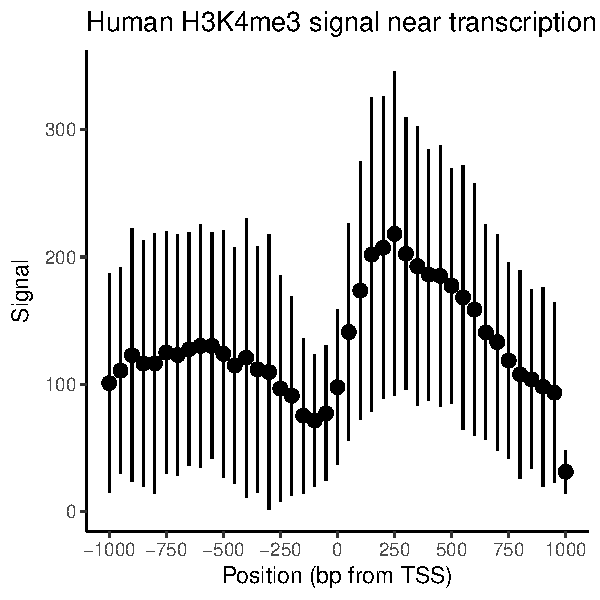
\includegraphics[width=\textwidth]{demo-tss-1.pdf}
        \label{fig:meta_gene_out}
    \end{subfigure}
\caption{\label{fig:your-figure}Meta-analysis of signals relative to genomic features with valr.}
\end{figure}


% See this guide for more information on BibTeX:
% http://libguides.mit.edu/content.php?pid=55482&sid=406343

% For more author guidance please see:
% https://f1000research.com/for-authors/article-guidelines/software-tool-articles


% When all authors are happy with the paper, use the 
% ‘Submit to F1000RESEARCH' button from the menu above
% to submit directly to the open life science journal F1000Research.

% Please note that this template results in a draft pre-submission PDF document.
% Articles will be professionally typeset when accepted for publication.

% We hope you find the F1000Research Overleaf template useful,
% please let us know if yo\begin{Shaded}

\begin{Shaded}
\begin{Highlighting}[]
\KeywordTok{library}\NormalTok{(dplyr)}
\KeywordTok{library}\NormalTok{(valr)}
\KeywordTok{library}\NormalTok{(R.utils)}
\KeywordTok{library}\NormalTok{(curl)}
\KeywordTok{library}\NormalTok{(ggplot2)}
\KeywordTok{library}\NormalTok{(gridExtra)}
\end{Highlighting}
\end{Shaded}

\subsection{Get the public datasets from
UCSC}\label{get-the-public-datasets-from-ucsc}


\begin{Shaded}
\begin{Highlighting}[]
\NormalTok{DMSO_treated<-}\KeywordTok{read_bed}\NormalTok{(}\StringTok{'http://hgdownload.soe.ucsc.edu/goldenPath/hg19/encodeDCC/wgEncodeHaibMethylRrbs/wgEncodeHaibMethylRrbsA549Dm002p7dHaibSitesRep1.bed.gz'}\NormalTok{, }\DataTypeTok{n_fields=}\DecValTok{6}\NormalTok{, }\DataTypeTok{skip=}\DecValTok{1}\NormalTok{)}
\end{Highlighting}
\end{Shaded}

\begin{Shaded}
\begin{Highlighting}[]
\NormalTok{untreated<-}\KeywordTok{read_bed}\NormalTok{(}\StringTok{'http://hgdownload.soe.ucsc.edu/goldenPath/hg19/encodeDCC/wgEncodeHaibMethylRrbs/wgEncodeHaibMethylRrbsAg04449UwSitesRep1.bed.gz'}\NormalTok{, }\DataTypeTok{n_fields=}\DecValTok{6}\NormalTok{, }\DataTypeTok{skip=}\DecValTok{1}\NormalTok{)}
\end{Highlighting}
\end{Shaded}

To view the data

\begin{Shaded}
\begin{Highlighting}[]
\KeywordTok{head}\NormalTok{(untreated)}
\end{Highlighting}
\end{Shaded}

\begin{verbatim}
#> # A tibble: 6 x 6
#>   chrom start   end           name score strand
#>   <chr> <int> <int>          <chr> <chr>  <chr>
#> 1  chr1 10785 10786 AG04449_0__JS_     1      +
#> 2  chr1 10788 10789 AG04449_0__JS_     1      +
#> 3  chr1 10794 10795 AG04449_0__JS_     1      +
#> 4  chr1 10810 10811 AG04449_0__JS_     1      +
#> 5  chr1 10812 10813 AG04449_0__JS_     1      +
#> 6  chr1 10815 10816 AG04449_0__JS_     1      +
\end{verbatim}

\subsection{Examine regions that are different and regions that
intersect}\label{examine-regions-that-are-different-and-regions-that-intersect}

\begin{Shaded}
\begin{Highlighting}[]
\NormalTok{different_region<-}\KeywordTok{bed_subtract}\NormalTok{(DMSO_treated,untreated, }\DataTypeTok{any=}\OtherTok{FALSE}\NormalTok{)}
\KeywordTok{dim}\NormalTok{(different_region)}
\end{Highlighting}
\end{Shaded}

\begin{verbatim}
#> [1] 278241      6
\end{verbatim}

\begin{Shaded}
\begin{Highlighting}[]
\NormalTok{intersect_region<-}\KeywordTok{bed_intersect}\NormalTok{(DMSO_treated,untreated, }\DataTypeTok{suffix=}\KeywordTok{c}\NormalTok{(}\StringTok{'.treated'}\NormalTok{,}\StringTok{'.untreated'}\NormalTok{))}
\KeywordTok{dim}\NormalTok{(intersect_region)}
\end{Highlighting}
\end{Shaded}

\begin{verbatim}
#> [1] 1576400      12
\end{verbatim}

\subsection{Plot the distribution of different regions and intersected
regions across
chromosomes}\label{plot-the-distribution-of-different-regions-and-intersected-regions-across-chromosomes}

\begin{Shaded}
\begin{Highlighting}[]
\NormalTok{p1<-}\KeywordTok{ggplot}\NormalTok{(}\DataTypeTok{data=}\NormalTok{different_region, }\KeywordTok{aes}\NormalTok{(}\DataTypeTok{x=}\NormalTok{chrom))+}\KeywordTok{geom_histogram}\NormalTok{(}\DataTypeTok{stat=}\StringTok{'count'}\NormalTok{, }\KeywordTok{aes}\NormalTok{(}\KeywordTok{factor}\NormalTok{(chrom), }\DataTypeTok{fill=}\StringTok{'differential methylation'}\NormalTok{))+}\KeywordTok{scale_fill_brewer}\NormalTok{(}\DataTypeTok{palette =} \StringTok{'Set2'}\NormalTok{)+}\KeywordTok{theme_minimal}\NormalTok{()+}\KeywordTok{ggtitle}\NormalTok{(}\StringTok{'Distribution of differential methylation across chromosomes'}\NormalTok{)+}\KeywordTok{theme}\NormalTok{(}\DataTypeTok{axis.text.x =} \KeywordTok{element_text}\NormalTok{(}\DataTypeTok{angle =} \DecValTok{45}\NormalTok{, }\DataTypeTok{hjust =} \DecValTok{1}\NormalTok{))}
\end{Highlighting}
\end{Shaded}

\begin{verbatim}
#> Warning: Ignoring unknown parameters: binwidth, bins, pad
\end{verbatim}

\begin{Shaded}
\begin{Highlighting}[]
\NormalTok{p2<-}\KeywordTok{ggplot}\NormalTok{(}\DataTypeTok{data=}\NormalTok{intersect_region, }\KeywordTok{aes}\NormalTok{(}\DataTypeTok{x=}\NormalTok{chrom))+}\KeywordTok{geom_histogram}\NormalTok{(}\DataTypeTok{stat=}\StringTok{'count'}\NormalTok{, }\KeywordTok{aes}\NormalTok{(}\KeywordTok{factor}\NormalTok{(chrom), }\DataTypeTok{fill=}\StringTok{'overlap methylation'}\NormalTok{))+}\KeywordTok{scale_fill_brewer}\NormalTok{(}\DataTypeTok{palette =} \StringTok{'Spectral'}\NormalTok{)+}\KeywordTok{theme_minimal}\NormalTok{()+}\KeywordTok{ggtitle}\NormalTok{(}\StringTok{'Distribution of overlapping methylation across chromosomes'}\NormalTok{)+}\KeywordTok{theme}\NormalTok{(}\DataTypeTok{axis.text.x =} \KeywordTok{element_text}\NormalTok{(}\DataTypeTok{angle =} \DecValTok{45}\NormalTok{, }\DataTypeTok{hjust =} \DecValTok{1}\NormalTok{))}
\end{Highlighting}
\end{Shaded}

\begin{verbatim}
#> Warning: Ignoring unknown parameters: binwidth, bins, pad
\end{verbatim}

\begin{Shaded}
\begin{Highlighting}[]
\KeywordTok{grid.arrange}\NormalTok{(p1, p2, }\DataTypeTok{ncol =} \DecValTok{1}\NormalTok{, }\DataTypeTok{nrow =}\DecValTok{2}\NormalTok{)}
\end{Highlighting}
\end{Shaded}
\begin{figure}
\begin{center}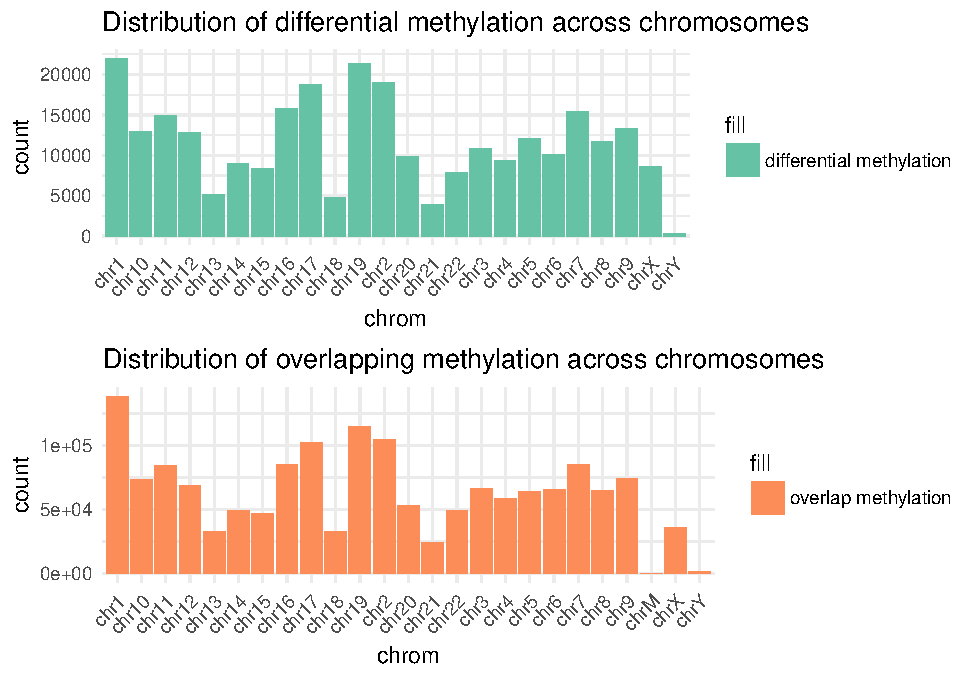
\includegraphics{unnamed-chunk-8-1} \end{center}
\end{figure}


\end{document}